% Copyright (c) 2017-2019 Matematyka dla Ciekawych Świata (http://ciekawi.icm.edu.pl/)
% Copyright (c) 2017-2019 Robert Ryszard Paciorek <rrp@opcode.eu.org>
% 
% MIT License
% 
% Permission is hereby granted, free of charge, to any person obtaining a copy
% of this software and associated documentation files (the "Software"), to deal
% in the Software without restriction, including without limitation the rights
% to use, copy, modify, merge, publish, distribute, sublicense, and/or sell
% copies of the Software, and to permit persons to whom the Software is
% furnished to do so, subject to the following conditions:
% 
% The above copyright notice and this permission notice shall be included in all
% copies or substantial portions of the Software.
% 
% THE SOFTWARE IS PROVIDED "AS IS", WITHOUT WARRANTY OF ANY KIND, EXPRESS OR
% IMPLIED, INCLUDING BUT NOT LIMITED TO THE WARRANTIES OF MERCHANTABILITY,
% FITNESS FOR A PARTICULAR PURPOSE AND NONINFRINGEMENT. IN NO EVENT SHALL THE
% AUTHORS OR COPYRIGHT HOLDERS BE LIABLE FOR ANY CLAIM, DAMAGES OR OTHER
% LIABILITY, WHETHER IN AN ACTION OF CONTRACT, TORT OR OTHERWISE, ARISING FROM,
% OUT OF OR IN CONNECTION WITH THE SOFTWARE OR THE USE OR OTHER DEALINGS IN THE
% SOFTWARE.

\documentclass{pdfBooklets}

\title{Linux i sieci: Sieci komputerowe}
\author{%
	Projekt ,,Matematyka dla Ciekawych Świata'',\\
	Robert Ryszard Paciorek\\\normalsize\ttfamily <rrp@opcode.eu.org>
}
\date  {2019-05-05}

\makeatletter\hypersetup{
	pdftitle = {\@title}, pdfauthor = {\@author}
}\makeatother

\usepackage[ampersand]{easylist}
\usepackage{paracol}

\begin{document}

\maketitle

\begin{teacherOnly}
	\begin{easylist}[itemize]
	& kto ma w domu telefon stacjonarny (taki klasyczny, analogowy)?
	& kto wie jak on działa?
	&& (to nam się przyda)
	& jak działa internet?
	& w jaki sposób dane są przesyłane z jednego komputera na drugi?
	&& pakiety
	& skąd wiedzą gdzie mają trafić?
	&& adresy, przełączanie pakietów vs łączy
	\end{easylist}
\end{teacherOnly}

% BEGIN: Sieci - intro
\section{Podstawy TCP/IP}

Sieci komputerowe działają na zasadzie przesyłania informacji w postaci porcji, z których każda posiada co najmniej informację o adresie odbiorcy (zwykle też nadawcy), nazywanych ramkami lub pakietami. Kierowanie pakietów w odpowiednie miejsce odbywa się na podstawie adresu pakietu i nie jest związane z fizycznym zestawianiem łącza pomiędzy nadawcą a odbiorcą - każdy pakiet jest kierowany niezależnie, a w ramach pojedynczego łącza (kanału transmisji) mogą być przekazywane pakiety adresowane do różnych odbiorców. Nazywane jest to komutacją pakietów, w odróżnieniu od komutacji łącza (która występowała np. w klasycznej, analogowej telefonii, gdzie przekaźniki w centralach dokonywały zestawienia połączeń elektrycznych między dwoma aparatami telefonicznymi).

\subsection{Struktura warstwowa}

Komunikacja sieciowa typowo posiada strukturę warstwową. W modelu OSI wyróżnia się 7 warstw:
\begin{enumerate}
	\item fizyczną (pierwszą) definiującą aspekty związane z fizycznym przesyłem sygnału takie jak częstotliwości radiowe, poziomy napięć, etc.;
		określa sposób transmisji kolejnych bajtów
	\item łącza danych (drugą) definiującą aspekty związane z formatem ramki, protokoły ustalania zasad dostępu do medium transmisyjnego, itd.;
		określa sposób transmisji porcji danych pomiędzy hostami w jednej sieci
	\item sieciową (trzecią) definiującą aspekty związane z formatem pakietu, adresacją i zasady routingu umożliwiające zapewnienie łączności pomiędzy różnymi sieciami;
		określa sposoby transmisji porcji danych pomiędzy sieciami
	\item transportową (czwartą) odpowiedzialną za podział strumienia na porcje informacji, kontrolę nad poprawnością transmisji, adresację usług w ramach hosta
	\item sesji (piątą)
	\item prezentacji (szóstą)
	\item aplikacji (siódmą)
\end{enumerate}
W modelu TCP/IP wyróżnia się 4 warstwy:
\begin{enumerate}
	\item Dostępu do sieci - obejmującą warstwy 1 i 2 modelu OSI
	\item Internetu - obejmującą warstwę 3 modelu OSI
	\item Transportową - obejmującą warstwę 4 modelu OSI
	\item Aplikacji - obejmującą warstwy 5, 6 i 7 modelu OSI
\end{enumerate}

Z punktu widzenia modelu TCP/IP można powiedzieć o enkapsulacji danych kolejnych warstw w ramach warstwy niższej, czyli "surowe" dane (np. strona HTML) obudowywane są strukturą opisywaną przez warstwę aplikacji (np. nagłówkami HTTP), następnie całość ta umieszczana jest w polu danych pakietu warstwy transportowej (np. TCP), ten z kolei w polu danych pakietu IP (warstwy sieciowej), na koniec pakiet IP jest umieszczany w polu danych ramki warstwy dostępu do sieci (np. ramki ethernetowej). W ramach podróży przez kolejne sieci pakiet IP jest wyjmowany i wkładany w kolejne ramki warstwy dostępu do sieci, na ogół tylko z niewielkimi ingerencjami w zawartość tego pakietu (prawie zawsze nie dochodzącymi do pola danych pakietu TCP lub datagramu UDP, czyli nie wykraczającymi poza warstwę 4 OSI).
% END: Sieci - intro

% BEGIN: adresacja IP
\subsection{Protokół IP}
Protokół IP (Internet Protocol) odpowiedzialny jest przede wszystkim za sposób adresacji hostów oraz reguły komutacji pakietów (routing). Jest on wspomagany przez kolejny protokół z tej rodziny - ICMP (Internet Control Message Protocol), którego zadaniem jest przekazywanie informacji kontrolnych np. o nieosiągalności hosta docelowego, odrzuceniu przetwarzania pakietu ze względu na zbyt dużą liczbę skoków (gdy wartość pola TTL z nagłówka IP wyniesie zero) a także pingi (zarówno żądanie jak i odpowiedź).

\teacher{ Pokazać i omówić dobry, kolorowy obrazek ilustrujący strukturę pakietu IPv4 i IPv6. }

\subsection{Adresacja IP}
Adresy hostów (nazywane adresami IP) są to 32-bitowe (w IPv4) lub 128-bitowe (w IPv6) liczby.
Adresy IPv4 zapisywane są najczęściej w notacji kropkowo-dziesiętnej, gdzie każdy bajt (ciąg 8 bitów) zapisywany jest jako liczba dziesiętna rozdzielana kropką od pozostałych. Adresy IPv6 zapisywane są zazwyczaj w notacji dwukropokowej, polegającej na zapisywaniu 16 bitowych części adresu liczbami szesnastkowymi oddzielanymi dwukropkiem, dodatkowo jeden ciąg zer (o długości będącej wielokrotnością 16 bitów) może być skompresowany (pominięty) co daje w zapisie dwa dwukropki \Verb$::$.

\subsubsection{Długość prefixu i maska}

\begin{teacherOnly}
	\begin{easylist}[itemize]
	& adres IP jest to liczba, a taki lub inny zapis służy naszej wygodzie
	& pierwsza część (najstarsze bity) określa adres sieci do której należy host, druga część adres hosta
	&& długość części określającej adres sieci określa jest za pomocą prefixu (który rozwinąć można do maski sieci)
	&&& wielkość prefixu określa ilość adresów dostępnych w danej sieci (dla prefixu o długości $n$ wynosi ona $2^{32-n}$ dla IPv4 i $n$ wynosi ona $2^{128-n}$)
	&&&& dla IPv4 użyteczna liczba adresów jest mniejsza o dwa: adres sieci (część hosta binarnie – same zera) i adres rozgłoszeniowy (część hosta – binarnie same jedynki)
	&& sieci mogą być grupowane w większe sieci
	& jak mając adres hosta i prefix ustalić adres sieci
	&& rozpiska na tablicy
	&& pokazać sipcalc
	&& porównywanie adresów sieci o nierównych maskach
	&&& pokazać ilustrację - kółko w kółku (każdy host widzi tylko piersze otaczające go kółko)
	\end{easylist}
\end{teacherOnly}

Adresy hostów grupuje się w adresy sieci, bazując na jednakowym (bitowo) początku takiego adresu (zwanym adresem sieci lub prefixem). Ilość bitów stanowiących adres sieci w danym adresie IP nazywana jest długością prefixu i zapisywana jest zazwyczaj po ukośniku. Np. zapis \Verb$2001:db8::a17/48$ oznacza że pierwsze 48 bity stanowią adres sieci a kolejne $128-48 = 80$ bitów stanowi adres hosta w tej sieci.

Długość prefixu jednoznacznie określa maskę danej podsieci, czyli liczbę odpowiadającą długości adresu (32 bity lub 128 bitów), złożoną z ciągu jedynek o długości prefixu oraz ciągu zer (o długości adresu hosta). W przypadku IPv4 spotykane jest także podawanie maski sieci w notacji kropkowo-dziesiętnej zamiast długości prefixu.

Sieć może zostać podzielona na mniejsze sieci (z większą wartością prefixu), jak też grupa sieci może zostać zagregowana w jedną większą ($2^n$ raza) sieć (z prefixem mniejszym o n). Agregacja hostów i sieci w większe całości jest wykorzystywana w mechanizmach routingu, co pozwala na redukcję wielkości tablic routingowych.

\subsubsection{Przynależność do sieci}
Adres sieci zapisuje się typowo z wyzerowanymi bitami stanowiącymi adres hosta (czyli po dokonaniu bitowego \emph{and} z maską danej sieci) oraz podaną informacją o długości prefixu, dla powyższego przykładu będzie to \Verb$2001:db8::/48$. Informacja taka jest wystarczająca do sprawdzenia czy dowolny inny adres IP należy do tej sieci czy nie.

\begin{CodeFrame*}[python][fontsize=\footnotesize]{}
from ipaddress import *

a1  = IPv6Address("2001:0db8::17:15")
aa1 = int(a1)
print("adress IPv6 jest 128 bitową liczbą całkowitą np.: " + str(a1) + " == " + hex(aa1))

n0  = IPv6Network("::/112");
m1  = n0.netmask
mm1 = int(m1)
p1  = n0.prefixlen

print("Maska podsieci IPv6 jest 128 bitową liczbą całkowitą np.: " + str(m1) + " == " + hex(mm1))
print("Jako że maska jest liczbą, która zapisana binarnie, zawsze zawiera ciągły ciąg bitów")
print("o wartości 1, a po nim ciągły ciąg bitów o wartości 0 (mogą być zerowej długości), to")
print("często stosowany jest zapis polegający na podawaniu długości prefiksu: /" + str(p1))
print("jest to ilość bitów o wartości 1 w masce, czyli im większy prefix tym mniejsza sieć.")

n1  = IPv6Network("2001:0db8::17:15/112", strict=False);
nn1 = int(n1.network_address)

print("Aby obliczyć adres sieci (czyli wspólną dla wszystkich hostów w danej sieci część")
print("adresu IP) należy wykonać binarny AND pomiędzy adresem IP hosta a maską podsieci.")
print("Dla powyższego przykładu:")
print(hex(mm1 & aa1) + " == " + str(n1) + " == " + hex(nn1))

# aby sprawdzić czy adres IP należy do danej sieci trzeba obliczyć adres sieci tego hosta
# w oparciu o maskę sieci którą sprawdzamy
def sprawdzSiec(n, a):
	nn = int(a) & int(n.netmask)
	if nn == int(n.network_address):
		print(str(a) + " należy do sieci " + str(n))
	else:
		print(str(a) + " NIE należy do sieci " + str(n))

sprawdzSiec(n1, IPv6Address("2001:0db8::17:ab13"))
sprawdzSiec(n1, IPv6Address("2001:0db8::13:a"))
\end{CodeFrame*}

\teacher{Wskazać różnice IPvXAddress vs IPvXNetwork oraz znaczenie strict=False. Pokazać kalkulowanie z palca.}

\begin{Zadanie}{}{}
Przeanalizuj powyższy kod programu. Zapoznaj się z dokumentacją modułu ipaddress\footnote{Można ją wyświetlić uruchamiając po jego zaimportowaniu: \python{help('ipaddress')}} i pamiętając, że adres IPv4 jest 32 bitową liczbą, zmodyfikuj ten program aby zamiast na adresach IPv6 działał na IPv4.
\end{Zadanie}

\subsection{Routing}
Router kieruje każdy z pakietów do kolejnego routera lub bezpośrednio do hosta docelowego na podstawie jego adresu docelowego i tablicy routingu. Tablica taka zawiera adresy sieci wraz z adresami następnych routerów do nich prowadzących bądź wskazaniem lokalnego interfejsu sieciowego poprzez który powinny być osiągalne hosty z danej sieci. W tym celu korzysta z sprawdzania przynależności adresu do sieci, w celu ustalenia adresu następnego routera i/lub interfejsu sieciowego na który ma zostać przekazany pakiet.

Tablica przeglądana jest od wpisów najbardziej precyzyjnych, czyli z największym prefixem do wpisów najbardziej ogólnych (ostatnim wpisem jest na ogół trasa domyślna czyli sieć ::/0 dla IPv6 lub 0.0.0.0/0 dla IPv4). Dzięki czemu jeżeli kilka wpisów (sieci) z tablicy routingu pasuje do adresu docelowego z nagłówka pakietu, wybierany jest wpis najbardziej precyzyjny (o najdłuższym prefixie), a pasująca do każdego adresu trasa domyślna wybierana jest tylko gdy nie ma żadnej lepszej. Może się zdarzyć że kilka wpisów (nawet z tą samą maską) pasuje do adresu docelowego hosta, w takiej sytuacji do wyboru ścieżki używane są inne dane z tablicy routingu (takie jak metryka).

Tablice routingu mogą zawierać wpisy dodawane statycznie (wpisane do konfiguracji danego urządzenia), jak też wpisy dodawane dynamicznie w oparciu o protokołu wymiany informacji routingowych (protokoły routingu) takie jak: IGRP, OSPF, BGP. Protokoły routingu dynamicznego mogą być wykorzystywane m.in. do rozkładania obciążenia na różne łącza, zapewnienia redundancji łącz, blokowania ataków (D)DoS.

Także każdy z hostów ma tablice routingu, typowo składa się z dwóch pozycji – trasy do sieci lokalnej (tej sieci z której adres posiada dany host) wskazującej bezpośrednio na urządzenie sieciowe oraz trasy domyślnej wskazującej na router zapewniający dostęp do innych sieci, nazywany bramką (gateway). Jeżeli router nie posiada adresu w tej samej sieci co host konieczna jest dodatkowa trasa wskazująca poprzez jakie urządzenie dostępny jest router domyślny.

Oprócz opisanego powyżej routingu unicastowego (kierowania do jednego odbiorcy) realizowane są także transmisje:
\begin{itemize}
	\item \emph{anycast} – do dowolnego / najbliższego hosta o danym adresie; zasadniczo jest to transmisja unicast, tyle że adres docelowy nie jest unikalny w skali globalnej a różne routery kieruje te pakiety do różnych hostów docelowych (typowo wybierając najbliższy taki host)
	\item \emph{multicast} – do grupy hostów, w tym wypadku (multicastowy) adres IP identyfikuje "kanał nadawczy" a nie unikalny host docelowy
	\item \emph{broadcast} – do wszystkich hostów (w ramach danej sieci – nie są routowne), transmisje rozgłoszeniowe można traktować jako szczególny przypadek transmisji multicastowych w których grupa multicastowa obejmuje wszystkie hosty (można je zastąpić takimi transmisjami multicastowymi)
\end{itemize}
% END: adresacja IP

\begin{teacherOnly}
	Pokazać i omówić ping i traceroute, wspomnieć o TTL.
	
	Można trochę rozwinąć temat adresacji:
	\begin{easylist}[itemize]
	& adresy IPv4
	&& Wyróżnia się także specjalne adresy (sieci) IP:
	&&& 0.0.0.0/0 – cały Internet
	&&& 127.0.0.0/8 (głownie adres 127.0.0.1) – pętla zwrotna (czyli komunikacja hosta lokalnego ze sobą)
	&&& 224.0.0.0/4 – multicast
	&&&& 232.0.0.0/8 – source-specific multicast (RFC 4607)
	&&&& 233.0.0.0/8 – adresy oparte na numerze AS, każdy posiadacz numeru AS może używać adresów 233.AS.AS.0/24 (RFC 3180)
	&&&& 234.0.0.0/8 – adresy oparte na unicastowej puli o prefixie /24 lub mniejszym, dla posiadacza a.b.c.0/24 dostępny jest adres multicastowy 234.a.b.c/32 (RFC 6034)
	&&&& 239.0.0.0/8 – adresy "prywatne" wykorzystywane w obrębie swojej "domeny" (RFC 2365)
	&&& adresy sieci prywatnych: 10.0.0.0 do 10.255.255.255, 172.16.0.0 do 172.31.255.255 i 192.168.0.0 do 192.168.255.255
	&& Można wspomnieć o tym że kiedyś stosowany był także podział na klasy sieci A, B i C odpowiadające maskom /8, /16 i /24 oraz klasy D, E i F (adresy 224.0.0.0 do 254.0.0.0)
	& adresy IPv6
	&& Wyróżnia się także specjalne adresy (sieci) IP:
	&&& ::/0 – cały Internet
	&&& ::1/128 – cały Internet
	&&& ff$yx$:: – multicast, gdzie $x$ odpowiada za zasięg który obejmuje transmisja multicastowa, $y$ koduje natomiast flagi dotyczące typu adresu (0=adres przydzielony na stałe przez IANA - dobrze znane usługi, 1=nie przydzielone stale, ...)
	&&&& ff3x::/104 – adresy multicast w oparciu o maksymalnie 64 bitowy prefiks sieci adresów unicast – dla sieci o adresie \Verb$prefix::/MM$ będzie to adres \Verb$ff3x:00mm:prefix:gropid$, gdzie \Verb$mm$ jest zapisaną w systemie szesnastkowym wartością MM, a \Verb$gropid$ identyfikatorem konkretnej grupy multicastowej (właściciel prefixu dysponuje $2^32$ grupami) (RFC3306).
	&&&& ff3x::/96 – source-specific multicast (nie jest to sprzeczne z powyższym, gdyż odpowiada mu przy \Verb$::/0$)
	&&& fe80:: – adresy linklocal tworzone w oparciu o MAC adres karty sieciowej,
	&&&& nie jest on routowany do sieci zewnętrznych, zawsze może być używany wewnątrz sieci lokalnej (ale wymaga jawnego określania interfejsu sieciowego dla pakietów adresowych na taki adres np. \Verb$ping6 fe80::f66d:4ff:fe4e:ade8%eth0$);
	&&&& adres taki (dla adresu MAC 11:22:33:44:55:66) będzie miał postać:\\ fe80::1{\bfseries 3}22:33{\bfseries FF}:{\bfseries FE}44:5566 (pierwsza część adresu MAC zwiększana jest o 2, w środku wstawiane jest FFFE).
	& broadcast
	&& występuje jedynie w IPv4, w IPv6 zastapiony multicastem:
	&&& ff0$x$::1 – wszystkie węzły
	&&& ff0$x$::2 – wszystkie routery
	&&& $x$ określa zasięg, np. x=2 w zakresie \emph{Link-Local}
	\end{easylist}
\end{teacherOnly}

% BEGIN: TCP / UDP
\section{Komunikacja TCP/IP}
W oparciu o protokół IP działają protokoły warstwy transportowej takie jak UDP, TCP, czy też (mniej znane protokoły czasu rzeczywistego, transmisji strumieniowych): RTP, RTCP i SCTP.
Najprostszym protokołem warstwy transmisji wydaje się być UDP, protokół ten umożliwia przesłanie informacji pomiędzy dwoma hostami IP i nie kontroluje on tego czy została ona przesłana poprawnie.
Natomiast TCP kontroluje to czy przesłana informacja dotarła do adresata i nie została uszkodzona, a w przypadku problemów informacja wysyłana jest ponownie. TCP w związku z tym w przeciwieństwie do UDP musi otworzyć połączenie i wykorzystywać je do kontroli poprawności przesłania informacji, wymaga zatem przesłania większej liczby pakietów (co może prowadzić do pewnych opóźnień itp).
W związku z tym TCP używany jest tam gdzie konieczna jest kontrola poprawności transmisji (oraz ponowne wysłanie zgubionego pakietu), UDP tam gdzie nie jest to potrzebne (a liczy się czas).

Dodatkowo zarówno UDP jak i TCP na każdym z hostów wyróżniają numeryczny identyfikator dla aplikacji/procesu/usługi będącego odbiorcą czy też nadawcą informacji zwany numerem portu.
% END: TCP / UDP

% BEGIN: Polularne usługi
\subsection{Polularne usługi}
W ramach sieci mogą być realizowane różne usługi w oparciu o różne protokoły warstwy aplikacyjnej. Standardowe usługi posiadają zdefiniowane domyślne adresy portów dla swoich protokołów. Wśród usług i protokołów sieciowych należy wymienić przynajmniej:
\begin{itemize}
	\item DNS (Domain Name System) - odpowiedzialny za system mapujący nazwy alfanumeryczne hostów na adresy IP.
		Domeny posiadają budowę hierarchiczną / drzewiastą (precyzja rośnie od prawej do lewej, a kolejne poziomy oddzielane są kropkami).
		\teacher{Wspomnieć o kropce kończącej nazwę domeny oraz o pliku \Verb$/etc/hosts$. Poopowiadać o typach rekordów także PTR. }
		Realizacja odpowiedzi na zapytanie DNS wygląda następująco:
		\begin{enumerate}
			\item host kieruje zapytanie do określonego w jego konfiguracji serwera "rozwijającego" DNS (DNS resolver),
			\item serwer taki sprawdza w swojej pamięci podręcznej czy zna odpowiedź na to zapytanie (i nie jest ona przeterminowana - nie upłynął czas TTL od odnalezienia), jeżeli nie ma jej w swojej pamięci to
			\item serwer taki zna adresy głównych serwerów DNS (root serwerów) zawierających informacje na temat serwerów obsługujących domeny najwyższego rzędu i kieruje do jednego z nich zapytanie o serwer obsługujący skrajnie prawą część adresu (np. \textit{.org}),
			\item do otrzymanego serwera kierowane jest zapytanie o większą część adresu (np. \textit{eu.org}),
			\item itd. aż do uzyskania odpowiedzi o pytany adres
		\end{enumerate}
	\item mechanizmy auto konfiguracji hostów - DHCP, rozgłaszanie informacji routingowej poprzez ICMPv6 (protokół warstwy 3)
	\item WWW - udostępnianie treści z użyciem protokołu HTTP
	\item pocztę elektroniczną - przesyłanie wiadomości (protokoły SMTP, IMAP, POP)
	\item komunikację natychmiastową i telefonię IP (protokoły SIP, XMPP, IAX)
	\item SSH - zdalny, szyfrowany dostęp do systemów IT, przesył plików oraz tunelowanie innych usług
\end{itemize}
% END: Polularne usługi

\begin{teacherOnly}
	Porozmawiać także o:
	\begin{easylist}[itemize]
	& standary Internetu - dokumenty RFC
	&& standardy de facto
	&& poważne i mniej (gołębie, ...)
	&& dość dobrze się czyta
	& czemu służą, jak działają (ogólnie) protokoły routingu dynamicznego
	& krótko o filtracji pakietów - iptables (jakiś przykład), łańcuchy, w oparciu o co można filtować
	\end{easylist}
	
	Można powiedzieć kilka słów o autkonfiguracji IPv6:
	
	Polega ona na tym że dla podsieci będących LAN'em przydzielana jest pula z maską /64 co umożliwia tworzenie unikalnych numerów IP w oparciu o (niepowtarzalne) numery sprzętowe MAC.
	64 bitowy prefiks sieci jest informacją rozgłaszaną przy pomocy ICMPv6 przez routery (mechanizm radvd), a host dokleja do niego część go identyfikującą związaną z adresem link-local.
	Radvd rozgłasza także informacje routingowe (takie jak adres bramy - dhcpv6 tego nie potrafi), niestety nie da się rozgłaszać w ten sposób innej od standardowej dla LAN długości prefixu.
\end{teacherOnly}

\subsection{Programowanie usług sieciowych}

\begin{teacherOnly}
	Na początek:
	\begin{easylist}[itemize]
	& zabawa netcat-em (serwer, klient) + tcpdum do podłuchiwania
	& kilka słów więcej o:
	&& HTTP (+ oglądanie WWW netcatem)
	&& SMTP (+ sesja SMTP netcatem)
	\end{easylist}
	
	Następnie \strong{krótkie} wprowadzenie systemowe:
	\begin{easylist}[itemize]
	& fork
	& komunikacja międzyprocesowa
	&& sygnały
	&&& poopowiadać o kill
	&&&& czy program może nie umrzeć?
	&&& wiele różnych sygnałów ...
	&& pamięć i semafory
	&&& poopwiadać o problemie if a==1: a=0
	& subprocess w pythonie
	& multiprocessing i lock w pythonie
	& funkcja \verb$getaddrinfo$
	\end{easylist}
\end{teacherOnly}


\subsubsection{wysyłanie danych po UDP}
\begin{CodeFrame*}[python]{}
import socket, sys

if len(sys.argv) != 3:
  print("USAGE: " + sys.argv[0] + " dstHost dstPort", file=sys.stderr)
  exit(1)

dstAddrInfo = socket.getaddrinfo(sys.argv[1], sys.argv[2])
dstAddrInfo = dstAddrInfo[0]
sfd = socket.socket(dstAddrInfo[0], socket.SOCK_DGRAM)

sfd.sendto("Ala ma kota".encode(), dstAddrInfo[4])
\end{CodeFrame*}

\subsubsection{odbiór danych po UDP}
\begin{CodeFrame*}[python]{}
import socket, sys

if len(sys.argv) != 2:
  print("USAGE: " + sys.argv[0] + " listenPort", file=sys.stderr)
  exit(1)

sfd = socket.socket(socket.AF_INET6, socket.SOCK_DGRAM)
sfd.setsockopt(socket.IPPROTO_IPV6, socket.IPV6_V6ONLY, 0)
sfd.bind(('::', int(sys.argv[1])))

while True:
  data, sAddr, = sfd.recvfrom(4096)
  print("odebrano od", sAddr, ":", data.decode());
\end{CodeFrame*}

\subsubsection{klient TCP}
\begin{CodeFrame*}[python]{}
import socket, select, sys

if len(sys.argv) != 3:
	print("USAGE: " + sys.argv[0] + " dstHost dstPort", file=sys.stderr)
	exit(1);

# struktura zawierająca adres na który wysyłamy
dstAddrInfo = socket.getaddrinfo(sys.argv[1], sys.argv[2], proto=socket.IPPROTO_TCP)

# mogliśmy uzyskać kilka adresów, więc próbujemy używać kolejnych do skutku
for aiIter in dstAddrInfo:
	try:
		print("try connect to:", aiIter[4])
		# utworzenie gniazda sieciowego ... SOCK_STREAM oznacza TCP
		sfd = socket.socket(aiIter[0], socket.SOCK_STREAM)
		# połączenie ze wskazanym adresem
		sfd.connect(aiIter[4])
	except:
		# jeżeli się nie udało ... zamykamy gniazdo
		if sfd:
			sfd.close()
		sfd = None
		# i próbujemy następny adres
		continue
	break;

if sfd == None:
	print("Can't connect", file=sys.stderr)
	exit(1);

# wysyłanie
sfd.sendall("Ala ma Kota\n".encode())

# czekanie na odbiór
rdfd, _, _ = select.select([sfd], [], [], 13.0)
if sfd in rdfd:
	d = sfd.recv(4096)
	print(d.decode())

# zamykanie połączenia
sfd.shutdown(socket.SHUT_RDWR)
sfd.close()
\end{CodeFrame*}

\subsubsection{serwer TCP}
\begin{CodeFrame*}[python]{}
import socket, select, signal, sys, os

MAX_CHILD = 5
QUERY_SIZE = 3
TIMEOUT = 13
BUF_SIZE = 4096

if len(sys.argv) != 2:
	print("USAGE: " + sys.argv[0] + " listenPort", file=sys.stderr)
	exit(1);

# obsługa sygnału o zakończeniu potomka
childNum = 0
def onChildEnd(s, f):
	print("odebrano sygnał o śmierci potomka")
	global childNum
	childNum -= 1
	os.waitpid(-1, os.WNOHANG);
signal.signal(signal.SIGCHLD, onChildEnd)

# utworzenie gniazd sieciowych ... SOCK_STREAM oznacza TCP
sfd_v4 = socket.socket(socket.AF_INET,  socket.SOCK_STREAM)
sfd_v6 = socket.socket(socket.AF_INET6, socket.SOCK_STREAM)

# ustawienie opcji gniazda ... IPV6_V6ONLY=1 wyłącza korzystanie
# z tego samego socketu dla IPv4 i IPv6
sfd_v6.setsockopt(socket.IPPROTO_IPV6, socket.IPV6_V6ONLY, 1)

# przypisanie adresów ...
# '0.0.0.0' oznacza dowolny adres IPv4 (czyli to samo co INADDR_ANY)
# '::' oznacza dowolny adres IPv6 (czyli to samo co in6addr_any)
sfd_v4.bind(('0.0.0.0', int(sys.argv[1])))
sfd_v6.bind(('::',      int(sys.argv[1])))

# określenie gniazd jako używanych do odbioru połączeń przychodzących
# (długość kolejki połączeń ustawiona na wartość QUERY_SIZE)
sfd_v4.listen(QUERY_SIZE)
sfd_v6.listen(QUERY_SIZE)

# funkcja zajmująca się odbieraniem połączeń i ich obsługą
def acceptConn(sfd):
	global childNum
	
	#  odebranie połączenia
	sfd_c, sAddr = sfd.accept()
	
	# weryfikacja ilości potomków
	if childNum >= MAX_CHILD:
		print("za dużo potomków - odrzucam połączenie od:", sAddr);
		sfd_c.send("Internal Server Error\r\n".encode())
		sfd_c.close()
		return
	
	# aby móc obsługiwać wiele połączeń rozgałęziamy proces
	pid = os.fork()
	if pid == 0:
		print("połączenie od:", sAddr)
		while True:
			# czekanie na dane z timeout'em
			# aby zabezpieczyć się przed atakiem DoS
			rd, _, _ = select.select([sfd_c], [], [], TIMEOUT)
			if sfd_c in rd:
				data = sfd_c.recv(BUF_SIZE)
				if not data:
					print("koniec połączenia od:", sAddr)
					break
				print("odebrano od", sAddr, ":", data.decode());
				sfd_c.send(data)
			else:
				print("timeout połączenia od:", sAddr)
				break
		# zamykanie połączenia
		sfd_c.shutdown(socket.SHUT_RDWR)
		sfd_c.close()
		sys.exit()
	else:
		childNum += 1

# czekanie na połączenia z użyciem select() w nieskończonej pętli
while True:
	sfd, _, _ = select.select([sfd_v4, sfd_v6], [], [])
	if sfd_v4 in sfd:
		acceptConn(sfd_v4)
	if sfd_v6 in sfd:
		acceptConn(sfd_v6)
\end{CodeFrame*}


\section{Ethernet}

\begin{teacherOnly}
	\begin{easylist}[itemize]
	& switche (wspomnieć o tym że kiedyś były też inne rozwiązania)
	&& switch softwerowy na linuxie
	&& zarządzanie switchem z poziomu OS (pokazać Junos OS)
	&&& wzmianka o BSD
	&&&& bardziej liberalna licencja, dłuższy rodowód, ...
	&&&& część rzeczy podobnie (shell, komendy posixowe)
	&&&& część rzeczy inaczej (konfiguracja ...)
	& pętle i STP
	& VLANy (tagowane i nie tagowane)
	& mediakonwertery i WDM
	& kable
	& wifi i hostap
	\end{easylist}
\end{teacherOnly}

% BEGIN: Warstwa sprzętowa
Od strony sprzętowej sieć składa z:
\begin{itemize}
	\item hostów stanowiących nadawców i odbiorców informacji
	\item urządzeń sieciowych pośredniczących w ich przekazywaniu, takich jak nadajniki, switche, mediakonwertery
	\item okablowania miedzianego bądź światłowodowego (jeżeli nie jest siecią bezprzewodową)
\end{itemize}

W przypadku sieci w standardzie Ethernet stosowane są 48 bitowe adresy MAC (pierwsza część identyfikuje producenta karty) oraz wspólny dla wszystkich odmian (przewodowych i bezprzewodowych) format ramki (określający położenie w ramce adresów, informacji dodatkowych oraz danych). Pakiety protokołu warstwy wyższej (np. pakiety IP wraz ich strukturą zawierającą adresy itd) z punktu widzenia ramki ethernetowej są danymi, w które ta warstwa nie wnika. Do mapowania adresów IP na adresy MAC wykorzystywany jest protokół ARP (dla IPv4) lub Neighbor Discovery (dla IPv6) - odbywa się to poprzez wysłanie ramki ethernetowej na adres rozgłoszeniowy (odbierany przez wszystkie hosty) z pytaniem o to jaki MAC adres ma host o podanym numerze IP.

Sieć ethernetowa typowo posiada strukturę wielokrotnej gwiazdy (drzewa), w węzłach której stosowane są switche. Kierują one ramki do odpowiednich gałęzi na podstawie adresu docelowego i wpisów w tablicy adresów MAC, utworzonej w oparciu o źródłowe nadawców przechodzących przez dany switch ramek. W przypadku gdy adresu docelowego nie ma w tablicy ramka kierowana jest na wszystkie porty switcha z wyjątkiem tego na którym została odebrana. W taki sposób zawsze są też przesyłane ramki wysyłane na adres rozgłoszeniowy (bradcast).

\begin{teacherOnly}
Można wspomnieć że dawniej funkcję switchy pełniły (dzisiaj już nie spotykany) mostek (bridge) będący w zasadzie switchem o dwóch gniazdach.
Natomiast do łączenia kabli wykorzystywany był (także już nie spotykany) hub (koncentrator) który zapewniał że sygnał nadawany przez dowolny z hostów do niego podłączonych był odbierany przez wszystkie inne (poza nim samym) oraz wzmacniał sygnał. Występował także regenerator (repeater) wzmacniający sygnał i umożliwiający przekroczenie ograniczenia 100m.

Najprostszy hub to w zasadzie drabinka oporników zapewniająca że po pełnym obiegu mamy oporność nieskończonej linii (100omów).
Można obyć się nawet bez żadnego huba, a jedynie z wykorzystaniem zwykłego trójnika (tutaj komputery wpięte w gniazdka trójnika się nie widzą - widzą tylko ten po drugiej stronie, a w komunikacji dużą rolę odgrywa protokół CSMA/CD).
\end{teacherOnly}

Ethernet pozwala na wirtualne podzielenie pojedynczej sieci lokalnej na wiele niezależnych (nie komunikujących się ze sobą w warstwie ethernetu) sieci, nazywanych VLAN. Działanie tego mechanizmu opiera się na zastosowaniu zarządzalnych switchy, które programowo mogą być dzielone na części zapewniające separację ruchu poszczególnych VLANów. Ponadto wybrane porty takiego switcha mogą być przypisane do różnych części (celem udostępnienia do innego switcha lub hosta kilku sieci wirtualnych), w takim przypadku do ramek ethernetowych wysyłanych tym portem dodawana jest informacja do którego VLANu należą (dwu bajtowy numer), a w przypadku ramek otrzymywanych na podstawie tego numeru odbywa się ich kierowanie do odpowiedniej "części" przełącznika (mówimy o VLANach tagowanych). Możliwe jest aby jeden wybrany VLAN na takim porcie był nie tagowany (do jego ramek nie będzie dodawany numer, a otrzymywane pakiety bez numeru będą kierowane do niego.

Ethernet pozwala również na grupowanie kilku portów w jeden port wirtualny (tzw port trunking / bonding) celem zwiększenia przepustowości lub niezawodności łącza. A dzięki zastosowaniu w różnych typach sieci ethernet tego samego formatu ramki możliwe jest też stosunkowo proste zmienianie medium transmisyjnego (np. z kabla miedzianego na światłowód) z użyciem media-konwerterów.

W przewodowych sieciach Ethernet wykrywaniem zajętości medium transmisyjnego oraz wykrywaniem kolizji zajmuje się protokół CSMA/CD (Carrier Sense Multiple Access with Collision Detection - wielodostęp z rozpoznawaniem stanu kanału oraz wykrywaniem kolizji). Przed rozpoczęciem nadawania stacja musi sprawdzić czy medium jest wolne, jeżeli tak może zacząć nadawać, jeżeli dwie stacje zaczną nadawać równocześnie zostaje to wykryte, obie przerywają nadawanie i wznawiają po losowym czasie. Jednak ze względu na stosowanie głównie połączeń punkt-punkt full-duplex (osobne przewody do nadawania i osobne do odbioru), co ogranicza tzw. domenę kolizji do pojedynczego hosta, protokół ten nie odgrywa obecnie szczególnie istotnej roli.
% END: Warstwa sprzętowa

\subsection{Kable}

Sieć ethernetowa wykorzystuje 8 żyłowe kable złożone z 4 par. Najpopularniejszym przewodem jest kabel UTP kategorii 5e, czyli nieekranowana skrętka pozwalająca na pracę z częstotliwością 100 MHz. W przypadku instalacji okablowania strukturalnego często stosowane są wyższe kategorie okablowania a także kable dodatkowo ekranowane. Ekran może obejmować osobno każdą parę, jak też może być wspólny dla całego przewodu, może być wykonany z folii lub siatki. Np. SF/FTP oznacza kabel z ekranem z siatki i folii (SF/), gdzie dodatkowo każda para jest ekranowana folią (FTP).

W ramach poszczególnych par realizowana jest transmisja różnicowa, czyli istotne jest napięcie pomiędzy przewodami w parze, a nie napięcie na danym przewodzie (w odniesieniu do jakiegoś zewnętrznego poziomu odniesienia).
Standard 100Mb/s (dokładniej 100BASE-TX) wykorzystuje jedynie dwie pary przewodów, standard 1Gb/s (1000BASE‑T) wykorzystuje wszystkie 4 pary przewodów.
Długość kabla pomiędzy dwoma urządzeniami nie powinna przekraczać 100 m.
Wykorzystywanie skręconych par przewodów (jeden skręt na 6-10 cm kabla) ma na celu eliminację zakłóceń transmisji - (w uproszczeniu) zakłócenia wchodzą tak samo na oba przewody i różnica miedzy nimi nie zmienia się.

Kable zakańczane są gniazdami bądź wtykami typu RJ-45 montowanymi według jednego z dwóch schematów kolorystycznych: EIA/TIA 568A lub 568B.
Pierwotnie (dla sieci 100Mb/s lub starszych) użycie różnych standardów na obu końcach kabla służyło stworzeniu kabla skrosowanego\footnote{Połączenie takie przy jednakowych urządzeniach, gdzie nadajnik i odbiornik trafia zawsze na te same piny, zamieniało na kablu nadajnik z odbiornikiem, umożliwiając transmisje między nimi. Aktualnie zdecydowana większość urządzeń obsługuje protokół \emph{Auto MDI-X}, który umożliwia automatyczne ustalenie na których pinach odbywa się nadawanie, a na których odbiór. W rzadkich przypadkach konieczne może być jednak zastosowanie kabla skrosowanego}.

\vspace{0.3cm}\noindent
\begin{minipage}{0.47\textwidth}
\begin{center}
{\noindent\large\bfseries EIA/TIA 568A}

{\noindent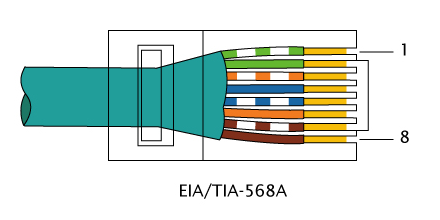
\includegraphics[width=0.7\textwidth,clip=true,trim={0, 4.5mm, 0, 0}]{RJ-45_TIA-568A_Right.png}}
\end{center}
\vspace{-0.3cm}

Kolejność przewodów we wtyczce/gnieździe:
\begin{enumerate}
	\item biało-zielony
	\item zielony
	\item biało-pomarańczowy
	\item niebieski
	\item biało-niebieski
	\item pomarańczowy
	\item biało-brązowy
	\item brązowy
\end{enumerate}
\end{minipage}
\hfill
\begin{minipage}{0.47\textwidth}
\begin{center}
{\noindent\large\bfseries EIA/TIA 568B}

{\noindent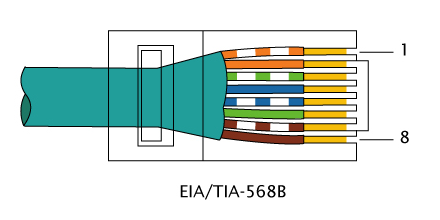
\includegraphics[width=0.7\textwidth,clip=true,trim={0, 4.5mm, 0, 0}]{RJ-45_TIA-568B_Right.png}}
\end{center}
\vspace{-0.3cm}

Kolejność przewodów we wtyczce/gnieździe:
\begin{enumerate}
	\item biało-pomarańczowy
	\item pomarańczowy
	\item biało-zielony
	\item niebieski
	\item biało-niebieski
	\item zielony
	\item biało-brązowy
	\item brązowy
\end{enumerate}
\end{minipage}
\vspace{0.3cm}

Wtyczki RJ-45 są wtyczkami zaciskanymi na przewodzie (bez konieczności odizolowywania żył). Gniazda RJ-45 najczęściej wykonywane są ze złączem typu IDC (Insulation Displacement Connector, KRONE/LSA) służącym do podłączenia przewodu również bez konieczności odizolowywania poszczególnych żył.

\section{Konfiguracja sieci w Linuxie}

Konfigurację interfejsów sieciowych w systemie Linux umożliwia polecenie \Verb$ip$. Przykłady użycia (ta lista w żaden sposób nie wyczerpuje dostępnych możliwości i dodatkowych opcji):
\begin{itemize}
	\item wyświetlanie i ustawianie adresów IP
		\begin{itemize}
			\item \Verb{ip addr} – wypisuje obecną konfigurację adresów i informacje o stanie interfejsu
			                 (\Verb{UP}/\Verb{DOWN} – interfejs włączony/wyłączony,
			                  \Verb{LOWER_UP}/\Verb{LOWER_DOWN} – link warsty niższej na interfejsie / jego brak)
			\item \Verb{ip addr add ADDRESS dev INTERFACE} – dodaje adres \Verb{ADDRESS} do interfejsu \Verb{INTERFACE}
			\item \Verb{ip addr del ADDRESS dev INTERFACE} – usuwa adres \Verb{ADDRESS} z interfejsu \Verb{INTERFACE}
		\end{itemize}
	\item włączanie i wyłaczanie interfejsów
		\begin{itemize}
			\item \Verb{ip link set INTERFACE up} / \Verb{ip link set INTERFACE down} – włączenie / wyłączenie interfejsu \Verb{INTERFACE}
			\item \Verb{ip link set INTERFACE address ADDRESS} – ustawienie adresu sprzętowego urządzenia \Verb{INTERFACE} na \Verb{ADDRESS}
		\end{itemize}
	\item konfiguracja tagowanych VLANów
		\begin{itemize}
			\item \Verb{ip link add link INTERFACE name INTERFACE.VLANID type vlan id VLANID} – dodanie interfejsu związanego z tagowanym VLANem o numerze \Verb{VLANID} na interfejsie \Verb{INTERFACE}, moduł 8021q powinien zostać załadowany automatycznie
			\item \Verb{ip link del INTERFACE.VLANID type vlan} – usunięcie interfejsu INTERFACE.VLANID (związanego z tagowanym VLANem VLANID na interfejsie INTERFACE
		\end{itemize}
	\item konfiguracja BRIDGE (programowego switcha)
		\begin{itemize}
			\item \Verb{ip link add INTERFACE type bridge} – dodanie interfejsu bridgowego o nazwie INTERFACE
			\item \Verb{ip link set SLAVE master INTERFACE}  – włączenie interfejsu SLAVE w skład bridgowego INTERFACE
			\item \Verb{ip link set SLAVE nomaster} - wyłaczenie interfejsu SLAVE z bridgowego
		\end{itemize}
	\item konfiguracja BONDów (interfejsów agregujących inne w grupę celem zwiększenia prędkości lub niezawodności)
		\begin{itemize}
			\item \Verb{ip link add INTERFACE type bond} – dodanie interfejsu bondingowego o nazwie INTERFACE
			\item \Verb{ip link set SLAVE master INTERFACE}  – włączenie interfejsu SLAVE w skład bondingu INTERFACE
			\item \Verb{ip link set SLAVE nomaster} - wyłaczenie interfejsu SLAVE z bondingu
		\end{itemize}
	\item konfiguracja routingu
		\begin{itemize}
			\item \Verb{ip route} \Verb{ip -6 route} – wyświetlanie informacji na temat tras routingowych dla IPv4 / IPv6
			\item \Verb{ip route add NETWORK via GATEWAY dev INTERFACE} – dodanie trasy routingowej do sieci \Verb{NETWORK} poprzez router o adresie \Verb{GATEWAY} na interfejsie \Verb{INTERFACE}
			\item \Verb{ip route del NETWORK via GATEWAY dev INTERFACE} – usunięcie trasy routingowej do sieci \Verb{NETWORK} ...
		\end{itemize}
\end{itemize}

Często dostępne są także klasyczne polecenia:
\begin{itemize}
	\item \Verb{ifconfig}
		włączanie i wyłączanie interfejsów sieciowych (up i down), ustawianie adresu IP i wyświetlanie informacji o interfejsach.
	\item \Verb{route}
		konfiguracja tras routingowych
	\item \Verb{vconfig}
		dodawanie i usuwanie obsługi wskazanych VLANów z danego interfejsu
	\item \Verb{brctl}
		konfiguracja programowego switcha ethernetowego pomiędzy interfejsmi (bridge)
	\item \Verb{ifenslave}
		konfiguracja bondów
\end{itemize}

Oprócz wyżej omówionej konfiguracji interfejsów i tras routingowych, często potrzebna jest konfiguracja jądrowych mechanizmów filtracji pakietów. Służą do tego komendy:
\begin{itemize}
	\item \Verb{iptables}
		konfiguracja filtrów działających na pakietach IP, filtracja może odbywać się m.in. w oparciu o źródłowe i docelowe adresy IP, numery portów, protokół warstwy transportowej, interfejsy oraz mechanizm śledzenia połączeń;
		umożliwia także konfigurację translacji adresów (NAT).
	\item \Verb{ebtables}
		konfiguracja filtrów działających na poziomie switcha ethernetowego, filtracja może odbywać się m.in. w oparciu o źródłowe i docelowe interfejsy i adresy sprzętowe.
	\item \Verb{arptables}
		konfiguracja filtrów związanych z protokołem ARP (zamiany adresów IP na adresy sprzętowe)
\end{itemize}

Ponaddto konieczne może być dokonywanie pewnych ustawień poprzez jądrowe systemy plików \Verb$/proc$ i \Verb$/sys$.
Najczęstszym przypadkiem jest włączenie przekazywania pakietów pomiędzy interfejsami poprzez:

\begin{minted}{bash}
for f in /proc/sys/net/ipv*/conf/*/forwarding; do echo 1 > $f; done
\end{minted}
(powyższy jednolinijkowiec włącza forwading pakietów IP dla IPv4 i IPv6 na wszystkich interfejsach)

\section{Zadania domowe}

\begin{Zadanie}{}{czy_w_sieci_ipv4} % [1pkt]
Ustal czy host o adresie IPv4 192.168.65.20 należy do sieci 192.168.33.15/19.
\end{Zadanie}


\begin{Zadanie}{}{czy_w_sieci_ipv6} % [1pkt]
Ustal czy host o adresie IPv6 2001:6a0:0:21::60:2 należy do sieci 2001:6a0:0:10::/58.
\end{Zadanie}


\begin{Zadanie}{}{adresy_serwerow_dns} % [1pkt]
Ustal adresy serwerów DNS posiadających informację o domenie \emph{gov}. Podaj polecenie którego użyłeś.
\end{Zadanie}

\begin{Zadanie}{}{} % [3pkt]
Polecenie \Verb{ip r} pokazało następują tablicę routingu:

\begin{Verbatim}
default via 192.168.29.2 dev eth0.2 
192.168.29.192/27 dev eth0.2  proto kernel  scope link  src 192.168.29.193
172.16.16.0/27 via 172.16.18.2 dev tun5 
172.16.16.48/28 dev wlan0  proto kernel  scope link  src 172.16.16.49 
172.16.18.0/30 dev tun5  proto kernel  scope link  src 172.16.18.1 
192.168.29.0/24 dev eth0  proto kernel  scope link  src 192.168.29.1 
\end{Verbatim}
Ustal trasę (urządzenie którym zostanie wysłany pakiet oraz jeżeli jest potrzebny to adres routera do którego będzie przesyłany) dla następujacych adresów IP:
\begin{itemize}
	\item 8.8.8.8
	\item 192.168.29.202
	\item 172.16.16.15
\end{itemize}
\end{Zadanie}


\begin{Zadanie}{}{} % [4pkt]
Na zajęciach omawialiśmy serwer usługi "echo" (odsyłającej odebrane dane do nadawcy).
Poniżej znajduje się prykładowy kod wysyłający dane po UDP ("klient UDP") i odbierający dane po UDP ("serwer UDP").
W oparciu o te informacje napisz program realizujący funkcję serwera echo z użyciem UDP.\\
\emph{Jeżeli nie lubisz Pythona program może być w C.}
\end{Zadanie}

\begin{Zadanie}{}{}
Zapoznaj się z RFC1924 i napisz program konweryjący adresy IPv6 pomiędzy notacją dwukropkową a noatacją base-85 zgodną z tą specyfikacją.
\end{Zadanie}

\rozwiazania

\copyrightFooter{
	© Matematyka dla Ciekawych Świata, 2017-2018.\\
	© Robert Ryszard Paciorek <rrp@opcode.eu.org>, 2003-2019.\\
	Wykorzystano grafiki należące do domeny publicznej.\\
	Kopiowanie, modyfikowanie i redystrybucja dozwolone pod warunkiem zachowania informacji o autorach.
}
\end{document}
